\documentclass[11pt, oneside]{article} 
\usepackage{geometry}
\geometry{letterpaper} 
\usepackage{graphicx}
	
\usepackage{amssymb}
\usepackage{amsmath}
\usepackage{parskip}
\usepackage{color}
\usepackage{hyperref}

\graphicspath{{/Users/telliott_admin/Tex/png/}}
% \begin{center} 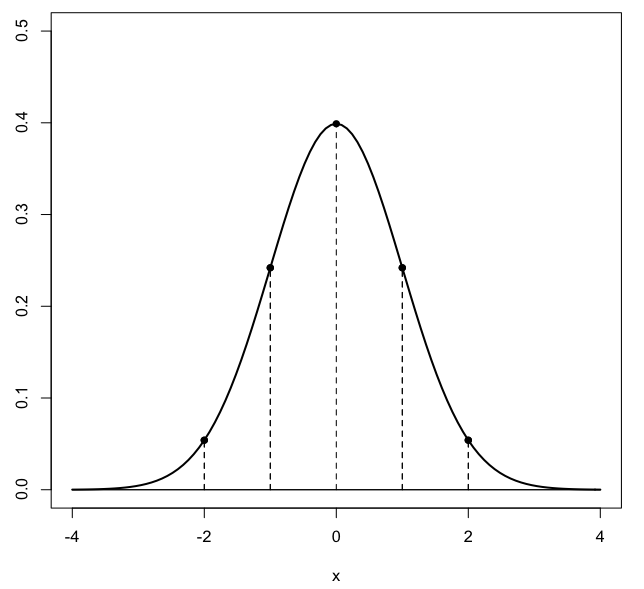
\includegraphics [scale=0.4] {gauss3.png} \end{center}

\title{Least squares}
\date{}

\begin{document}
\maketitle
\Large

We want to decide how to draw the best line through a bunch of data points,  In the figure below, given the three data points, we need to find the slope and y-intercept of a line that maximizes the fit according to some idea.  The criterion that is used most often is called "least squares."  In this method, the line that minimizes the (sum of the squares of the) vertical distance between each point and the line is chosen as the "best fit."

\begin{center}
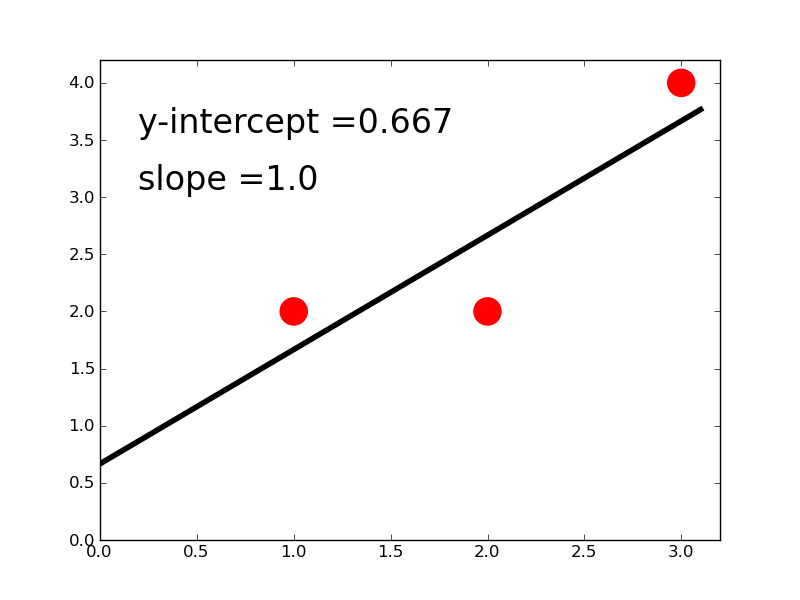
\includegraphics [scale=0.4] {regress.png}
\end{center}
As usual, the equation of the line is in the form y = slope times x + intercept.  We will call these C and D:
\[ y = C + Dx \]
We need to find C and D.  Let's write out the distances between the data points and our (as yet undetermined) line.  The points are (1,2), (2,2), and (3,4).  The magnitude of the "error" at times 1, 2 and 3 is the difference between the value on the line and the value we actually observed.
\[ e1 = C + (1)D - 2 \]
\[ e2 = C + (2)D - 2 \]
\[ e3 = C + (3)D - 4 \]
The sum of the squared errors is
\[ S = (C + D - 2)^2 + (C + 2D - 2)^2 +  (C + 3D - 4)^2 \]
Note that this is a function of both C and D, so the procedure will be to take the two partial derivatives, and set them both equal to zero.
\[ \frac{\partial S}{\partial C} =  2(C + D - 2) + 2(C + 2D - 2) + 2 (C + 3D - 4)\]
In the second equation, we will pick up coefficients of D by the chain rule
\[ \frac{\partial S}{\partial D} =  2(C + D - 2) + (2) 2(C + 2D - 2) + (3) 2 (C + 3D - 4)\]
Let's work with the first equation.  
\[ 2(C + D - 2) + 2(C + 2D - 2) + 2 (C + 3D - 4) = 0 \]
\[ C + D - 2 + C + 2D - 2 + C + 3D - 4 = 0 \]
\[ 3C + 6D - 8 = 0 \]
\[ 3C + 6D - 8 = 0 \]
\[ 3C = -6D + 8 \]
Leave it that way for a second.  Now look at equation 2.
\[ \frac{\partial S}{\partial D} =  2(C + D - 2) + (2) 2(C + 2D - 2) + (3) 2 (C + 3D - 4)\]
\[ 2(C + D - 2) + (2) 2(C + 2D - 2) + (3) 2 (C + 3D - 4) = 0 \]
\[ C + D - 2 + 2C + 4D - 4 + 3C + 9D - 12 = 0 \]
\[ 6C + 14D - 18 = 0 \]
Substitute for 3C into equation 2
\[ 6C + 14D - 18 = 2(-6D + 8) + 14D - 18 = 0 \]
\[ 2D - 2 = 0 \]
\[ D = 1 \]
\[ 3C = -6D + 8 = 2 \]
\[ C = \frac{2}{3}  \]
If we calculate the actual errors we have
\[ e1 = \frac{2}{3} + 1 - 2 = -\frac{1}{3} \]
\[ e2 = \frac{2}{3} + 2 - 2 = \frac{2}{3}  \]
\[ e3 = \frac{2}{3} + 3 - 4 = -\frac{1}{3} \]
Notice that the sum of the errors is equal to 0.  This is always true of these solutions.

There are better formulas for a real problem.  For example, using $\mu$ for the mean
\[ slope = A = \frac{\mu(xy) - \mu(x)\mu(y)}{\mu(x^2) - \mu(x)^2} \]
\[ intercept = B = \mu(y) - A \ \mu(x) \]
Notice that the line goes through the $\mu(x), \mu(y)$.  For our problem, we calculate
\[ \mu(x) = 2, \ \ \ \ \mu(y) = \frac{8}{3} \]
\[ \mu(xy) =\frac{(1*2 + 2*2 + 3*4)}{3} = \frac{18}{3}  \]
\[ \mu(x)\mu(y) = \frac{16}{3} \]
\[ \mu(x^2) = \frac{1 + 4 + 9}{3} = \frac{14}{3} \]
\[ \mu(x)^2 = 4 \]
\[ A = \frac{\mu(xy) - \mu(x)\mu(y)}{\mu(x^2) - \mu(x)^2} =\frac{ \frac{18}{3} - \frac{16}{3}}{\frac{14}{3} - \frac{12}{3} }= 1 \]
\[ B = \mu(y) - A \ \mu(x) = \frac{8}{3} - 2 = \frac{2}{3} \]
Just for fun, we can check using R:

\begin{verbatim}
> x = c(1,2,3)
> y = c(2,2,4)
> fit <- lm(y ~ x)
> fit

Call:
lm(formula = y ~ x)

Coefficients:
(Intercept)            x  
     0.6667       1.0000  
\end{verbatim}

Here is a derivation of the formula.  We write the sum of the squared deviations as
\[ D = f(a,b) = \sum \ [ \ y_i - (ax_i + b) \ ]^2 \] 
Take the partial derivative with respect to each variable and set it equal to 0
\[ \frac{\partial D}{\partial a} = \sum \ [ \ y_i - (ax_i + b) \ ](-x_i) = 0 \]
\[ \frac{\partial D}{\partial b} = \sum \ [ \ y_i - (ax_i + b) \ ](-1) = 0 \] 
Rearranging the first equation
\[ \frac{\partial D}{\partial a} = \sum -x_iy_i + ax_i^2 + bx_i  = 0 \]
Now the second
\[ \frac{\partial D}{\partial b} = \sum \ x_ia + b - y_i = 0 \]
To give two equations
\[  \sum x_i^2a + \sum x_ib = \sum  x_iy_i  \]
\[ \sum x_ia + \sum b  = \sum y_i \] 
This is just a 2 x 2 linear system in a and b.  Time for Cramer's Rule!
The denominator is 
\[  N \sum x_i^2 - (\sum x_i)^2  \] 
So for the slope a and intercept b we get:

\[ a = \frac{N \sum  x_iy_i - \sum x_i \sum y_i }{N \sum x_i^2 - (\sum x_i)^2} \]
\[ b =   \frac{\sum y_i \sum x_i^2 -  \sum x_i \sum  x_iy_i }{N \sum x_i^2 - (\sum x_i)^2}   \]

All terms can be converted to means by dividing by N.  Each double sum needs two divisions by N, which makes the leading N's disappear.

\[a = \frac {\mu_{xy} - \mu_x \mu_y }{ \mu_{x^2} - (\mu_x)^2 }  \] 
\[b = \frac {\mu_{y} \mu_{x^2} - \mu_x \mu_{xy} }{ \mu_{x^2} - (\mu_x)^2 }  \] 

A little algebra will confirm that 
\[ b = \mu_y - a \mu_x \]
as we had above.  Again, the point $(\mu_x,\mu_y)$ satisfies the equation of the line for the "best fit."  It is on the line.
\end{document}  